\lab{Python}{Intro to pandas I}{Intro to pandas I}
\objective{Become acquainted with the data structures and tools that pandas offers for data analysis.}
\label{lab:pandas1}

In volumes 1 and 2, we solved data problems primarily using NumPy and SciPy.
While extremely flexible and useful tools, these libraries lack some of the high-level 
data-analytic abstractions present in other popular data packages like R and Stata.
We now turn our attention to \emph{pandas}, a Python library that is more specifically built
for data analysis.

\section*{Data Structures in pandas}
Just as NumPy is built on the \li{ndarray} data structure suited for efficient scientific
and numerical computation, pandas is centered around a handful of core data structures
custom built for data analysis. These data structures include the \li{Series}, \li{DataFrame},
and \li{Panel}, which correspond roughly to one, two, and three-dimensional arrays.
We will explore the first two data structures in some detail.
The interested reader can learn more about the \li{Panel} data structure (the least-used one in pandas) in the online documentation.

\subsection*{Series}
The \li{Series} is a one-dimensional array with labeled entries. The values of the array may be
any data type, including integers, strings, or general Python objects. Further, the array
need not be homogeneous. That is, it can hold values of different data types. Together,
the array values are referred to as the \emph{data} of the \li{Series}.
The labels must consist of hashable types, and are most commonly integers or strings.
Together, the labels are referred to as the \emph{index} of the \li{Series}.

Thus, a \li{Series} consists of data and an index. The most basic way to initialize such an object
is as follows:
\begin{lstlisting}
>>> import pandas as pd
>>> s = pd.Series(data, index=index)
\end{lstlisting}
We don't need to explicitly define the index. The default index is simply \li{np.arange(len(data))}.

For example, we can create a Series containing the integers from 9 down to 0:
\begin{lstlisting}
>>> s1 = pd.Series(range(9, -1, -1))
>>> s1.values    #the data
array([9, 8, 7, 6, 5, 4, 3, 2, 1, 0])
>>> s1.index     #the labels
Int64Index([0, 1, 2, 3, 4, 5, 6, 7, 8, 9], dtype='int64')
>>> s1           #left column is index, right column is data
0    9
1    8
2    7
3    6
4    5
5    4
6    3
7    2
8    1
9    0
dtype: int64
\end{lstlisting}

Here is an example where we create customized labels:
\begin{lstlisting}
>>> import numpy as np
>>> data = np.random.randn(3)
>>> index = ['first', 'second', 'third']
>>> s2 = pd.Series(data, index=index)
>>> s2
first     1.661255
second   -0.033570
third    -2.185991
dtype: float64
\end{lstlisting}

We can create a \li{Series} having constant values in the following manner:
\begin{lstlisting}
>>> val = 4     #desired constant value of Series
>>> n = 6       #desired length of Series
>>> s3 = pd.Series(val, index=range(n))
>>> s3
0    4
1    4
2    4
3    4
4    4
5    4
dtype: int64
\end{lstlisting}

It is also possible to use a Python dictionary when creating a \li{Series}:
\begin{lstlisting}
>>> d = {'e1': 93, 'e2': 95, 'e3': 87, 'e4': 82, 'e5': 94}
>>> s4 = pd.Series(d)
>>> s4
e1    93
e2    95
e3    87
e4    82
e5    94
dtype: int64
\end{lstlisting}
Note that we didn't need to specify the index; the keys of the dictionary are used as the index for the \li{Series}.
There are many more ways to create Series objects.
For a more complete discussion of how to create Series objects, see the online documentation.

\begin{problem}
Create the following pandas \li{Series}.

\begin{itemize}
\item Constant array with value -3, length 5. Labels should be the first five positive even integers.

\item Data is given by the dictionary \li{\{'Bill': 31, 'Sarah': 28, 'Jane': 34, 'Joe': 26\}}.
\end{itemize}
\end{problem}

\subsection*{DataFrame}
The \li{DataFrame} data structure is a two-dimensional generalization of the \li{Series}. It can be viewed
as a tabular structure with labeled rows and columns. The row labels are collectively called the
index, and the column labels are collectively called the columns. An individual column in a
\li{DataFrame} object is a \li{Series}.

There are many ways to initialize a \li{DataFrame}. In the following, we build a \li{DataFrame} out of a
dictionary of \li{Series}.
\begin{lstlisting}
>>> x = pd.Series(np.random.randn(4), ['a', 'b', 'c', 'd'])
>>> y = pd.Series(np.random.randn(5), ['a', 'b', 'd', 'e', 'f'])
>>> d = {1: x, 2: y}
>>> df1 = pd.DataFrame(d)
>>> df1
	        1	        2
a	-0.924259	-0.708301
b	 0.767422	-2.214516
c	 0.399212	      NaN
d	 0.130365	-2.352364
e	      NaN	 0.789419
f	      NaN	-0.859482
\end{lstlisting}
Note that the index of this \li{DataFrame} is the union of the index of \li{Series} \li{x} and that of \li{Series} \li{y}.
The columns are given by the keys of the dictionary \li{d}. Since \li{x} doesn't have a label \li{e}, the
value in row \li{e}, column \li{1} is \li{NaN}. This same reasoning explains the other missing values as well.
Note that if we take the first column of the \li{DataFrame} and drop the missing values, we recover the \li{Series} \li{x}:
\begin{lstlisting}
>>> x == df1[1].dropna()
a    True
b    True
c    True
d    True
dtype: bool
\end{lstlisting}

\begin{warn}
A Pandas \li{DataFrame} cannot be sliced the same way a NumPy array could.
Notice how we just used \li{df1[1]} to access the first \emph{column} of the the \li{DataFrame} \li{df1}.
We will discuss this in more detail later on.
\end{warn}

We can also initialize a \li{DataFrame} using a NumPy array, creating custom row and column labels:
\begin{lstlisting}
>>> data = np.random.random((3, 4))
>>> pd.DataFrame(data, index=['A', 'B', 'C'], columns=range(1, 5))

            1	        2	        3	        4
A	 0.065646	 0.968593	 0.593394	 0.750110
B	 0.803829	 0.662237	 0.200592	 0.137713
C	 0.288801	 0.956662	 0.817915	 0.951016
3 rows     4 columns
\end{lstlisting}
As with Series, if we don't specify the index or columns, the default is \li{range(n)}, where \li{n}
is either the number of rows or columns.

It is also possible to create multi-indexed arrays, for example:
\begin{lstlisting}
>>> grade=['eighth', 'ninth', 'tenth']
>>> subject=['math', 'science', 'english']
>>> myindex = pd.MultiIndex.from_product([grade, subject], names=['grade', 'subject'])
>>> myseries = pd.Series(np.random.randn(9), index=myindex)
>>> myseries
grade   subject
eighth  math       1.706644
        science   -0.899587
        english   -1.009832
ninth   math       2.096838
        science    1.884932
        english    0.413266
tenth   math      -0.924962
        science   -0.851689
        english    1.053329
dtype: float64
\end{lstlisting}

Multi-indexing is visually convenient, but not strictly necessary for most applications.
The interested reader is invited to explore the documentation to learn more.

\section*{Data I/O}
Being able to import and export data is a fundamental skill in data science. Unfortunately, with the
multitude of data formats and conventions out there, importing data can often be a tricky task. The pandas library
seeks to reduce some of the difficulty by providing file readers for various types of formats, including
CSV, Excel, HDF5, SQL, JSON, HTML, or pickle files.

Because CSV files are one of the most popular file formats for exchanging data, we will explore the
\li{read_csv} function in more detail. To learn to read other types of file formats, see the online pandas documentation.
To read a CSV data file into a \li{DataFrame}, call the \li{read_csv} function with the path to the CSV file,
along with the appropriate keyword arguments. Below we list some of the most important keyword arguments:
\begin{itemize}
\item \li{delimiter}:
This argument specifies the character that separates data fields, often a comma or a whitespace character.

\item \li{header}:
The row number (starting at 0) in the CSV file that contains the column names.

\item \li{index_col}:
If you want to use one of the columns in the CSV file as the index for the \li{DataFrame},
set this argument to the desired column number.

\item \li{skiprows}:
If an integer $n$, skip the first $n$ rows of the file, and then start reading in the data. If a list
of integers, skip the specified rows.

\item \li{names}:
If the CSV file does not contain the column names, or you wish to use other column names, specify them
in a list assigned to this argument.

\end{itemize}
There are several other keyword arguments, but this should be enough to get you started.

When you need to save your data, pandas allows you to write to several different file formats.
A typical example is the \li{to_csv} function method attached to \li{Series} and \li{DataFrame} objects,
which writes the data to a CSV file.
Keyword arguments allow you to specify the separator character, omit writing the columns names or index,
and other options. The code below demonstrates its typical usage:
\begin{lstlisting}
>>> df.to_csv("my_df.csv")
\end{lstlisting}

\section*{Viewing and Accessing Data}

Once we have our data ready to go in pandas, how can we interact with it?
In this section we will explore some elementary access, plotting, and querying techniques that enable us to maneuver through
and gain insight into our data.

\subsection*{Basic Data Access}
Some of the basic slicing paradigms in NumPy carry over to pandas. 
For example, we can slice a \li{Series} using the usual syntax:
\begin{lstlisting}
>>> s = pd.Series(np.random.randn(5))
>>> s[1:3]

1    3.188112
2    0.080191
dtype: float64
\end{lstlisting}
Notice that both the data and the index are sliced in this manner.

Likewise, we can slice the rows of a \li{DataFrame} much as with a two-dimensional NumPy array:
\begin{lstlisting}
>>> df = pd.DataFrame(np.random.randn(4, 2), index=['a', 'b', 'c', 'd'], columns = ['I', 'II'])
>>> df[:2]

          I        II
a  0.758867  1.231330
b  0.402484 -0.955039

[2 rows x 2 columns]
\end{lstlisting}

More generally, we can select subsets of the data using the \li{.iloc} and \li{.loc} methods.
The \li{.loc} method selects rows and columns based on their labels, while the \li{.iloc} method
selects them based on their integer position.
It is interesting to know that accessing Series and DataFrames using these indexing operations is more efficient than using bracket indexing.
Since Series and DataFrames can be accessed by a numerical index or by label, the bracket indexing has to check many cases before it can determine how to slice the data structure.
By using \li{loc}/\li{iloc} explicitly, you bypass all of the extra checks.
\begin{lstlisting}
>>> # select rows a and c, column II
>>> df.loc[['a','c'], 'II']

a    1.231330
c    0.556121
Name: II, dtype: float64

>>> # select last two rows, first column
>>> df.iloc[-2:, 0]

c   -0.171938
d   -0.814336
Name: I, dtype: float64
\end{lstlisting}
Finally, a column of a \li{DataFrame} may be accessed using simple square brackets and the name of the column:
\begin{lstlisting}
>>> # get second column of df
>>> df['II']

a    1.231330
b   -0.955039
c    0.556121
d    0.173165
Name: II, dtype: float64
\end{lstlisting}

All of these techniques for getting subsets of the data may also be used to set subsets of the data:
\begin{lstlisting}
>>> # set second columns to zeros
>>> df['II'] = 0
>>> df['II']

a    0
b    0
c    0
d    0
Name: II, dtype: int64
\end{lstlisting}

\subsection*{Plotting}
Plotting is often a much more effective way to view and gain understanding of a dataset than simply
viewing the raw numbers. Fortunately, pandas interfaces well with matplotlib, allowing relatively
painless data visualization.

We start by plotting a \li{Series}. Doing so is easy, as the \li{Series} object is equipped with its own plot
function.
Let's start with visualizing a simple random walk. By way of background, a \emph{random walk} is a
stochastic process used to model a non-deterministic path through some space. It is a useful construct in
many fields and can be used to explain things like the motion of a molecule as it travels through a liquid to modeling or the fluctuations
of stock prices. Here we will simulate a one-dimensional symmetric random walk on the integers, which can be
described as follows.
\begin{enumerate}
  \item Start at 0.
  \item Flip a fair coin.
  \item If heads, move one unit to the right. Otherwise, move one unit to the left.
  \item Go to Step 2.
\end{enumerate}
How can we simulate this random walk efficiently? Note that the walk is really characterized by the outcomes
of the coin flip. If we represent heads by the number $1$ and tails by $-1$, then our position at a given moment
is just the cumulative sum of all previous outcomes. Below, we simulate a sequence of coin flips, build the
resulting random walk, and plot the outcome.
\begin{lstlisting}
>>> import matplotlib.pyplot as plt
>>> N = 1000        # length of random walk
>>> s = np.zeros(N)
>>> s[1:] = np.random.binomial(1, .5, size=(N-1,))*2-1 #coin flips
>>> s = pd.Series(s)
>>> s = s.cumsum()  # random walk
>>> s.plot()
>>> plt.ylim([-50, 50])
>>> plt.show()
\end{lstlisting}

The random walk is shown in Figure \ref{fig:PandasRandomWalk}.

\begin{figure}
\centering
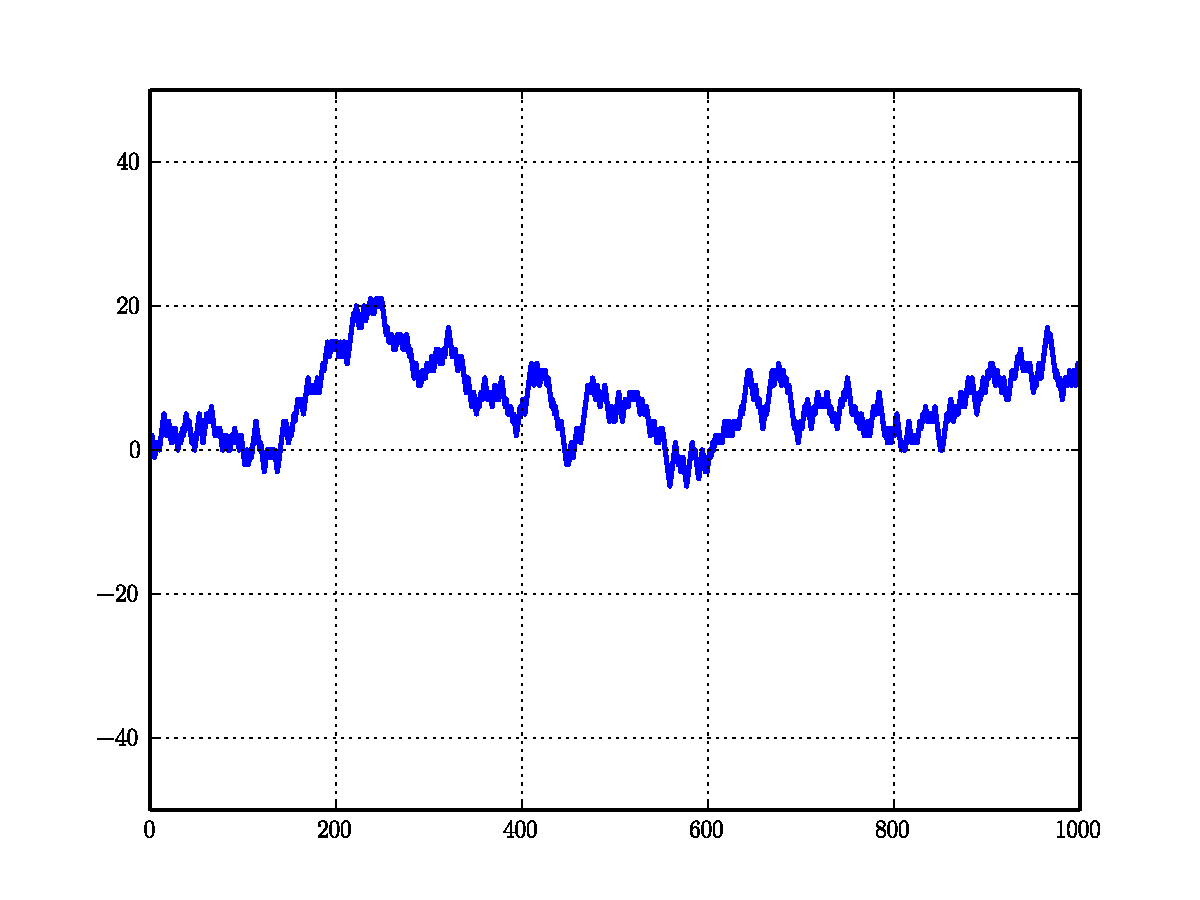
\includegraphics[width=.7 \textwidth]{randomWalk.pdf}
\caption{Random walk of length 1000.}
\label{fig:PandasRandomWalk}
\end{figure}

\begin{problem}
Create five random walks of length 100, and plot them together.

Next, create a ``biased'' random walk by changing the coin flip probability of head from 0.5 to 0.51.
Plot this biased walk with lengths 100, 10000, and then 100000. Notice the definite trend that emerges.
Your results should be comparable to those in Figure \ref{pandas:biasedRandomWalk}.
\end{problem}

\begin{figure}
\centering
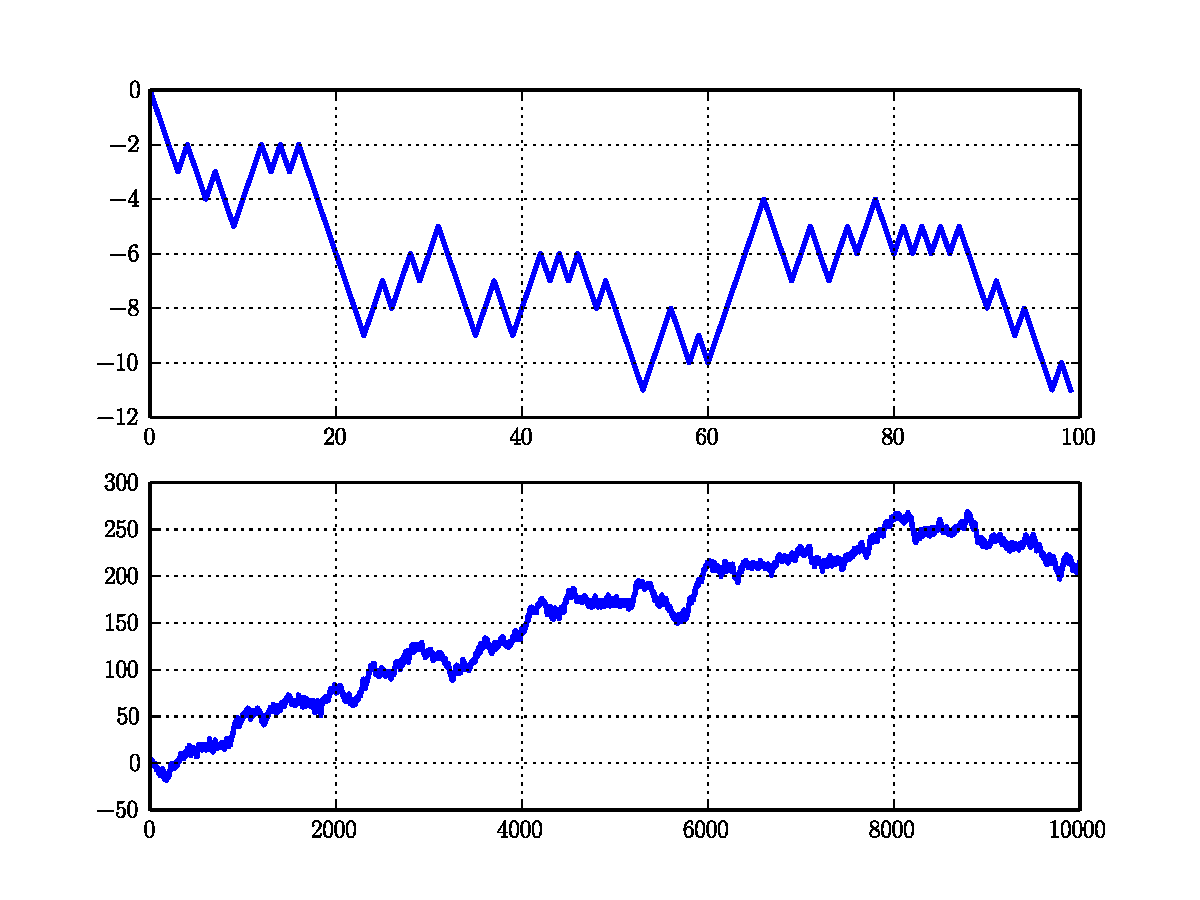
\includegraphics[width=.7 \textwidth]{biasedRandomWalk.pdf}
\caption{Biased random walk of length 100 (above) and 10000 (below).}
\label{pandas:biasedRandomWalk}
\end{figure}

Using \li{DataFrames}, one can also plot one column against another.

\begin{lstlisting}
>>> xvals = pd.Series(np.sqrt(np.arange(1000)))
>>> yvals = pd.Series(np.random.randn(1000).cumsum())
>>> df = pd.DataFrame({'xvals': xvals, 'yvals': yvals})
>>> df.plot(x='xvals', y='yvals') # specify x and y values
>>> plt.show()
\end{lstlisting}

The result is displayed in Figure \ref{pandas:dfPlot}.

\begin{figure}
\centering
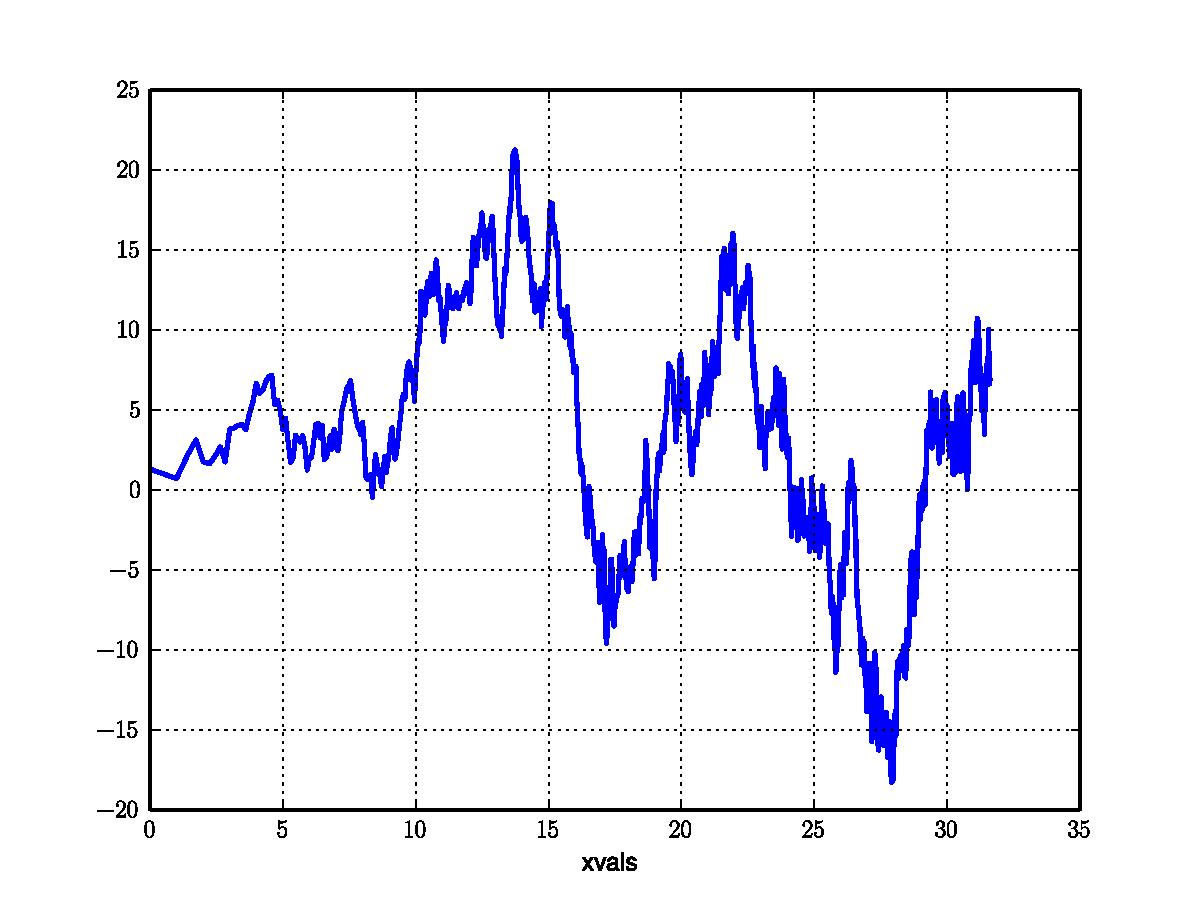
\includegraphics[width=.7 \textwidth]{dfPlot.pdf}
\caption{ Graph generated when one coordinate is taken from the xvals column and the other from the yvals column.}
\label{pandas:dfPlot}
\end{figure}

A variety of other types of plots are possible. One of the more useful plots when trying to estimate or
visualize the distribution of data is a histogram. The code listed below demonstrates how to generate
a histogram for each column in a \li{DataFrame}, with the result shown in Figure \ref{fig:PandasHistogram}.

\begin{lstlisting}
>>> col1 = pd.Series(np.random.randn(1000))         #normal distribution
>>> col2 = pd.Series(np.random.gamma(5, size=1000)) #gamma distribution
>>> df = pd.DataFrame({'normal': col1, 'gamma': col2})
>>> df.hist()
>>> plt.plot()
\end{lstlisting}

\begin{figure}
\centering
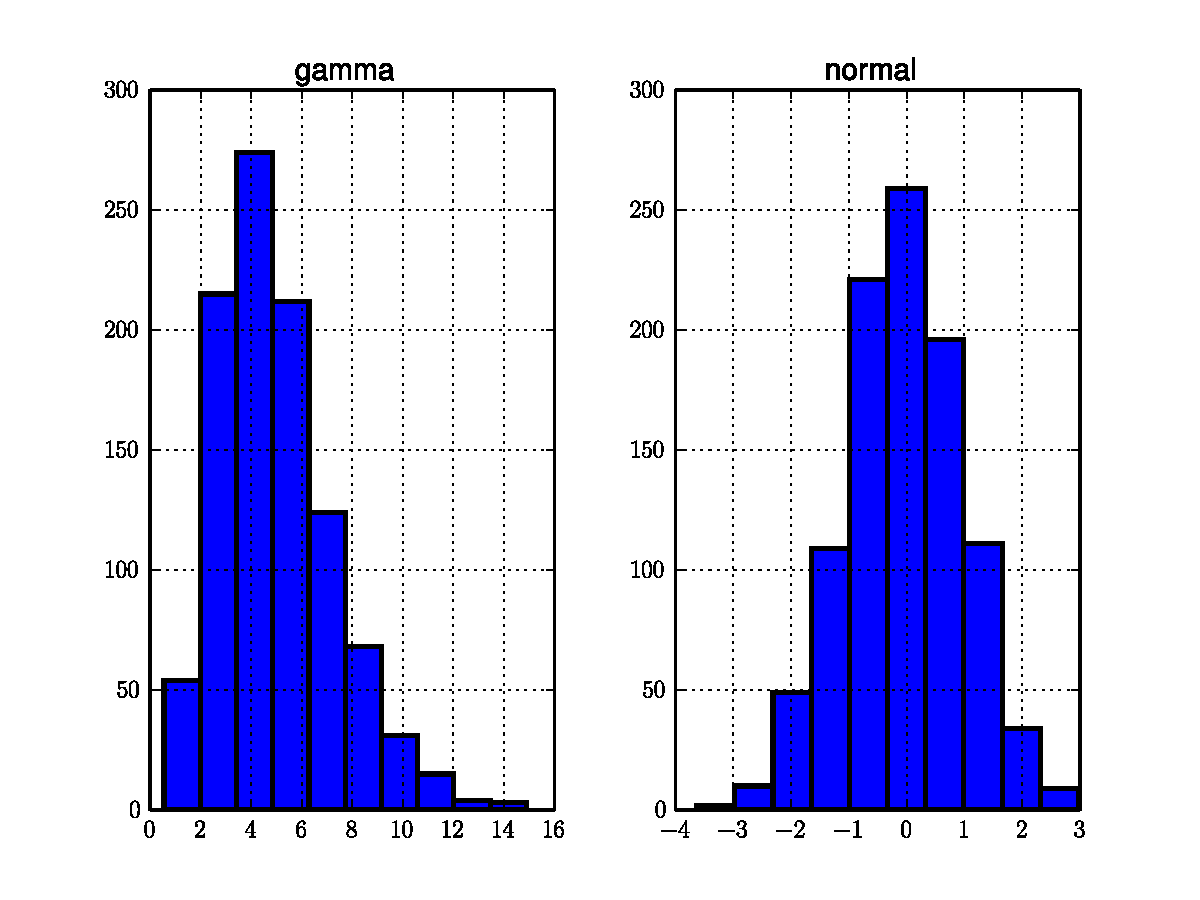
\includegraphics[width=.7 \textwidth]{histogram.pdf}
\caption{Histogram of two columns of a DataFrame.}
\label{fig:PandasHistogram}
\end{figure}

\subsection*{SQL Operations in pandas}
The \li{DataFrame}, being a tabular data structure, bears an obvious resemblance to a typical relational
database table. SQL is the standard for working with relational databases, and in this section we will
explore how pandas accomplishes some of the same tasks as SQL. The SQL-like functionality of pandas is
one of its biggest advantages, since it can eliminate the need to switch between programming languages
for different tasks. Within pandas we can handle both the querying \emph{and} data analysis.

For the following examples, we will use this data:
\begin{lstlisting}
>>> #build toy data for SQL operations
>>> name = ['Bill', 'Alice', 'Joe', 'Jenny', 'Ted', 'Taylor', 'Tracy', 'Morgan', 'Liz']
>>> sex = ['M', 'F', 'M', 'F', 'M', 'F', 'M', 'M', 'F']
>>> age = [20, 21, 18, 22, 19, 20, 20, 19, 20]
>>> rank = ['Sp', 'Se', 'Fr', 'Se', 'Sp', 'J', 'J', 'J', 'Se']
>>> ID = range(9)
>>> aid = ['y', 'n', 'n', 'y', 'n', 'n', 'n', 'y', 'n']
>>> GPA = [3.8, 3.5, 3.0, 3.9, 2.8, 2.9, 3.8, 3.4, 3.7]
>>> mathID = [0, 1, 5, 6, 3]
>>> mathGd = [4.0, 3.0, 3.5, 3.0, 4.0]
>>> major = ['y', 'n', 'y', 'n', 'n']
>>> studentInfo = pd.DataFrame({'ID': ID, 'Name': name, 'Sex': sex, 'Age': age, 'Class': rank})
>>> otherInfo = pd.DataFrame({'ID': ID, 'GPA': GPA, 'Financial_Aid': aid})
>>> mathInfo = pd.DataFrame({'ID': mathID, 'Grade': mathGd, 'Math_Major': major})
\end{lstlisting}

Before querying our data, it is important to know some of its basic properties, such as
number of columns, number of rows, and the datatypes of the columns. This can be done
by simply calling the \li{info} method on the desired \li{DataFrame}:
\begin{lstlisting}
>>> mathInfo.info()
<class 'pandas.core.frame.DataFrame'>
Int64Index: 5 entries, 0 to 4
Data columns (total 3 columns):
Grade         5 non-null float64
ID            5 non-null int64
Math_Major    5 non-null object
dtypes: float64(1), int64(1), object(1)
\end{lstlisting}

Now let's look at the pandas equivalent of some SQL SELECT statements.
\begin{lstlisting}
>>> # SELECT ID, Age FROM studentInfo
>>> studentInfo[['ID', 'Age']]

>>> # SELECT ID, GPA FROM otherInfo WHERE Financial_Aid = 'y'
>>> otherInfo[otherInfo['Financial_Aid']=='y'][['ID', 'GPA']]

>>> # SELECT Math_Major, COUNT(*) FROM mathInfo GROUP BY Math_Major
>>> print mathInfo.groupby('Math_Major').size()
\end{lstlisting}

\begin{problem}
The example above shows how to implement a simple WHERE condition, and it is easy
to have a more complex expression. Simply enclose each simple condition by parentheses,
and use the standard boolean operators \li{\&} (AND), \li{\|} (OR), and \li{\~} (NOT) to
connect the conditions appropriately. Use pandas to execute the following query:
\begin{lstlisting}[language=SQL]
SELECT ID, Name from studentInfo WHERE Age > 19 AND Sex = 'M'
\end{lstlisting}
\end{problem}

Next, let's look at JOIN statements. In pandas, this is done with the \li{merge} function,
which takes as arguments the two \li{DataFrame} objects to join, as well as keyword arguments specifying
the column on which to join, along with the type (left, right, inner, outer).

\begin{lstlisting}
>>> # SELECT * FROM studentInfo INNER JOIN mathInfo ON studentInfo.ID = mathInfo.ID
>>> pd.merge(studentInfo, mathInfo, on='ID') # INNER JOIN is the default
   Age Class  ID    Name Sex  Grade Math_Major
0   20    Sp   0    Bill   M    4.0          y
1   21    Se   1   Alice   F    3.0          n
2   22    Se   3   Jenny   F    4.0          n
3   20     J   5  Taylor   F    3.5          y
4   20     J   6   Tracy   M    3.0          n
[5 rows x 7 columns]

>>> # SELECT GPA, Grade FROM otherInfo FULL OUTER JOIN mathInfo on otherInfo.ID = mathInfo.ID
>>> pd.merge(otherInfo, mathInfo, on='ID', how='outer')[['GPA', 'Grade']]
   GPA  Grade
0  3.8    4.0
1  3.5    3.0
2  3.0    NaN
3  3.9    4.0
4  2.8    NaN
5  2.9    3.5
6  3.8    3.0
7  3.4    NaN
8  3.7    NaN
[9 rows x 2 columns]
\end{lstlisting}

\begin{problem}
Using a join operation, create a \li{DataFrame} containing the ID, age, and GPA of all male individuals.
You ought to be able to accomplish this in one line of code.
\end{problem}

\begin{comment}
This may be going into too much detail for an introductory lab...
It is sometimes desirable to join to DataFrames on their indexes rather than on a particular column.
The \li{join} method makes this operation convenient.
\begin{lstlisting}
>>> #create new DataFrame
>>> sibs = [0, 1, 0, 5, 2, 9]
>>> sibInfo = pd.DataFrame({'Siblings':sibs})
>>> sibInfo
   Siblings
0         0
1         1
2         0
3         5
4         2
5         9
[6 rows x 1 columns]

>>> #now join studentInfo with sibInfo
>>> studentInfo.join(sibInfo)
   Age Class  ID    Name Sex  Siblings
0   20    Sp   0    Bill   M         0
1   21    Se   1   Alice   F         1
2   18    Fr   2     Joe   M         0
3   22    Se   3   Jenny   F         5
4   19    Sp   4     Ted   M         2
5   20     J   5  Taylor   F         9
6   20     J   6   Tracy   M       NaN
7   19     J   7  Morgan   M       NaN
8   20    Se   8     Liz   F       NaN
[9 rows x 6 columns]
\end{lstlisting}
The default is a left join, but this can be altered.
When attempting to join to DataFrames that share common columns on their indexes,
we must rename the columns to avoid contradictions. We do this by simply appending
characters to the existing column names, specified by the \li{lsuffix} and \li{rsuffix}
parameters (for the left and right DataFrames, respectively).
\begin{lstlisting}
>>> #join studentInfo and mathInfo on indexes
>>> studentInfo.join(mathInfo, lsuffix='_left', rsuffix='_right', how='inner')
   Age Class  ID_left   Name Sex  Grade  ID_right Math_Major
0   20    Sp        0   Bill   M    4.0         0          y
1   21    Se        1  Alice   F    3.0         1          n
2   18    Fr        2    Joe   M    3.5         5          y
3   22    Se        3  Jenny   F    3.0         6          n
4   19    Sp        4    Ted   M    4.0         3          n
[5 rows x 8 columns]
\end{lstlisting}

The final SQL-like operation we will discuss is the UNION, or concatenation of DataFrames.
In the simplest setting, this operation is useful when we have two DataFrames that have the
same columns but possibly different rows.
\begin{lstlisting}
>>> #create another df holding more math info
>>> mathID2 = [0, 5, 2, 4]
>>> mathGd2 = [4.0, 3.5, 2.0, 3.0]
>>> major2 = ['y', 'y', 'n', 'y']
>>> mathInfo2 = pd.DataFrame({'Grade':mathGd2, 'ID':mathID2, 'Math_Major':major2})
>>> pd.concat([mathInfo, mathInfo2], ignore_index=True).drop_duplicates()
   Grade  ID Math_Major
0    4.0   0          y
1    3.0   1          n
2    3.5   5          y
3    3.0   6          n
4    4.0   3          n
7    2.0   2          n
8    3.0   4          y
[7 rows x 3 columns]
\end{lstlisting}
The \li{ignore_index=True} argument means we discard the indexes of the two input DataFrames and create
a new one for the concatenated DataFrame. The \li{drop_duplicates} method simply drops duplicate rows.
\end{comment}

Be aware that other types of SQL-like operations are also possible, such as UNION.
When you find yourself unsure of how to carry out a more involved SQL-like operation, the online
pandas documentation will be of great service.

\section*{Analyzing Data}
Although pandas does not provide built-in support for heavy-duty statistical analysis of data, there
are nevertheless many features and functions that facilitate basic data manipulation and computation,
even when the data is in a somewhat messy state. We will now explore some of these features.

\subsection*{Basic Data Manipulation}
Because the primary pandas data structures are subclasses of the \li{ndarray}, they are valid input
to most NumPy functions, and can often be treated simply as NumPy arrays. For example, basic
vectorized operations work just fine:
\begin{lstlisting}
>>> x = pd.Series(np.random.randn(4), index=['a', 'b', 'c', 'd'])
>>> y = pd.Series(np.random.randn(5), index=['a', 'b', 'd', 'e', 'f'])
>>> x**2
a    1.710289
b    0.157482
c    0.540136
d    0.202580
dtype: float64
>>> z = x + y
>>> z
a    0.123877
b    0.278435
c         NaN
d   -1.318713
e         NaN
f         NaN
dtype: float64
>>> np.log(z)
a   -2.088469
b   -1.278570
c         NaN
d         NaN
e         NaN
f         NaN
dtype: float64
\end{lstlisting}
Notice that pandas automatically aligns the indexes when adding two \li{Series} (or \li{DataFrames}),
so that the the index of the output is simply the union of the indexes of the two inputs. The default
missing value \li{NaN} is given for labels that are not shared by both inputs. 

It may also be useful to transpose \li{DataFrames}, re-order the columns or rows, or sort according to a 
given column. Here we demonstrate these capabilities:
\begin{lstlisting}
>>> df = pd.DataFrame(np.random.randn(4,2), index=['a', 'b', 'c', 'd'], columns=['I', 'II'])
>>> df
          I        II
a -0.154878 -1.097156
b -0.948226  0.585780
c  0.433197 -0.493048
d -0.168612  0.999194

[4 rows x 2 columns]

>>> df.transpose()
           a         b         c         d
I  -0.154878 -0.948226  0.433197 -0.168612
II -1.097156  0.585780 -0.493048  0.999194

[2 rows x 4 columns]

>>> # switch order of columns, keep only rows 'a' and 'c'
>>> df.reindex(index=['a', 'c'], columns=['II', 'I'])
         II         I
a -1.097156 -0.154878
c -0.493048  0.433197

[2 rows x 2 columns]

>>> # sort descending according to column 'II'
>>> df.sort(columns='II', ascending=False)
          I        II
d -0.168612  0.999194
b -0.948226  0.585780
c  0.433197 -0.493048
a -0.154878 -1.097156

[4 rows x 2 columns]
\end{lstlisting}

\subsection*{Basic Statistical Functions}
The pandas library allows us to easily calculate basic summary statistics of our data, 
useful when we want a quick description of the data. The \li{describe} function
outputs several such summary statistics for each column in a \li{DataFrame}:
\begin{lstlisting}
>>> df.describe()
              I        II
count  4.000000  4.000000
mean  -0.209630 -0.001308
std    0.566696  0.964083
min   -0.948226 -1.097156
25%   -0.363516 -0.644075
50%   -0.161745  0.046366
75%   -0.007859  0.689133
max    0.433197  0.999194

[8 rows x 2 columns]
\end{lstlisting}

Functions for calculating means and variances, the covariance and correlation matrices, and other 
basic statistics are also available. Below, we calculate the means of each row, as well as the
covariance matrix:
\begin{lstlisting}
>>> df.mean(axis=1)
a   -0.626017
b   -0.181223
c   -0.029925
d    0.415291
dtype: float64

>>> df.cov()
           I        II
I   0.321144 -0.256229
II -0.256229  0.929456

[2 rows x 2 columns]
\end{lstlisting}

\subsection*{Dealing with Missing Data}
Missing data is a ubiquitous problem in data science. Fortunately, pandas is particularly well-suited to 
handling missing and anomalous data. As we have already seen, the pandas default for a missing value is \li{NaN}. 
In basic arithmetic operations, if one of the operands is \li{NaN}, then the output is also \li{NaN}.
The following example illustrates this concept:
\begin{lstlisting}
>>> x = pd.Series(np.arange(5))
>>> y = pd.Series(np.random.randn(5))
>>> x.iloc[3] = np.nan
>>> x + y
0    0.731521
1    0.623651
2    2.396344
3         NaN
4    3.351182
dtype: float64
\end{lstlisting}
If we are not interested in the missing values, we can simply drop them from the data altogether:
\begin{lstlisting}
>>> (x + y).dropna()
0    0.731521
1    0.623651
2    2.396344
4    3.351182
dtype: float64
\end{lstlisting}

This is not always the desired behavior, however. It may well be the case that missing data actually corresponds to
some default value, such as zero. In this case, we can replace all instances of \li{NaN} with a specified value:
\begin{lstlisting}
>>> # fill missing data with 0, add
>>> x.fillna(0) + y
0    0.731521
1    0.623651
2    2.396344
3    1.829400
4    3.351182
dtype: float64
\end{lstlisting}

Other functions, such as \li{sum()} and \li{mean()} treat NaN as zero by default.
When dealing with missing data, make sure you are aware of the behavior of the pandas
functions you are using.

\begin{problem}
Using the dataset contained in the file \li{crime_data.txt} and the techniques learned in this lab, 
use pandas to complete the following.
\begin{itemize}
\item Load the data into a pandas \li{DataFrame}, using the column names in the file and the column titled
``Year'' as the index. Make sure to skip lines that don't contain data.

\item Insert a new column into the data frame that contains the crime rate by year (the ratio of ``Total'' column
to the ``Population'' column).

\item Plot the crime rate as a function of the year.

\item List the 5 years with the highest crime rate in descending order.

\item Calculate the average number of total crimes as well as burglary crimes between 1960 and 2012.

\item Find the years for which the total number of crimes was below average, but the number of burglaries
was above average.

\item Plot the number of murders as a function of the population.

\item Select the Population, Violent, and Robbery columns for all years in the 1980s, and save
this smaller data frame to a CSV file \li{crime_subset.txt}.
\end{itemize}
\end{problem}